\documentclass{standalone}
\usepackage[T1]{fontenc}
\usepackage[utf8]{inputenc}
\usepackage[usenames,dvipsnames]{xcolor}
\usepackage{tikz}
\usetikzlibrary{plotmarks}
\usetikzlibrary{shapes,snakes,arrows}
\begin{document}
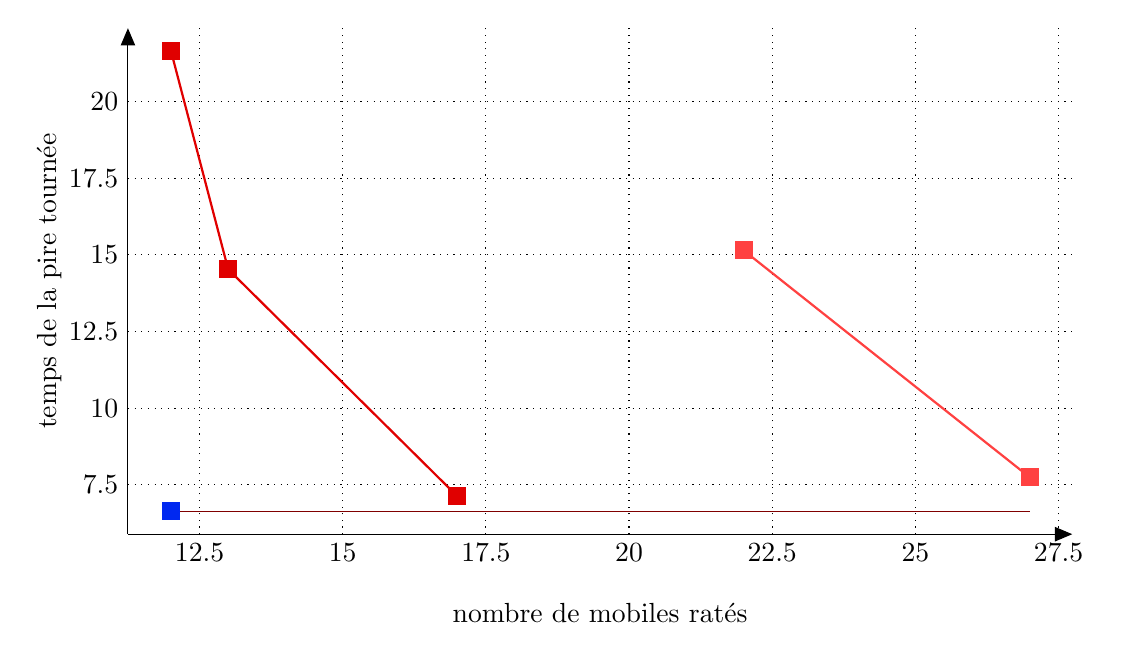
\begin{tikzpicture}[xscale=0.727273,yscale=0.389642]
\draw[xstep=2.5,ystep=2.5,thin,dotted,color=Black] (11.25,5.89481) grid (27.7393,22.3861);
\begin{scope}
  \clip (11.25,5.89481) rectangle (27.7393,22.3861);
  \definecolor{hvColor}{RGB}{128,0,0}
  \draw[color=hvColor, fill=hvColor, fill opacity=0.4] (12,6.64534) -- (12,6.64534) -| (27,6.64534) -- cycle;
  \definecolor{pLineColor}{RGB}{128,0,0}
  \definecolor{pPointColor}{RGB}{0,40,240}
  \draw[thick,color=pPointColor] (12,6.64534) node[draw,color=pPointColor,fill=pPointColor, inner sep = 0pt, minimum size=2mm] {};
  \definecolor{pLineColor}{RGB}{224,0,0}
  \definecolor{pPointColor}{RGB}{224,0,0}
  \draw[thick,color=pPointColor] (12,21.6559) node[draw,color=pPointColor,fill=pPointColor, inner sep = 0pt, minimum size=2mm] {} -- (13,14.5307) node[draw,color=pPointColor,fill=pPointColor, inner sep = 0pt, minimum size=2mm] {} -- (17,7.13526) node[draw,color=pPointColor,fill=pPointColor, inner sep = 0pt, minimum size=2mm] {};
  \definecolor{pLineColor}{RGB}{255,65,65}
  \definecolor{pPointColor}{RGB}{255,65,65}
  \draw[thick,color=pPointColor] (22,15.147) node[draw,color=pPointColor,fill=pPointColor, inner sep = 0pt, minimum size=2mm] {} -- (27,7.74618) node[draw,color=pPointColor,fill=pPointColor, inner sep = 0pt, minimum size=2mm] {};
\end{scope}
\draw[->,>=triangle 45] (11.25,5.89481) -- coordinate (x axis mid) (27.7393,5.89481);
\node[below=1cm,anchor=center] at (x axis mid) {nombre de mobiles ratés};
\foreach \x in {12.5,15,17.5,20,22.5,25,27.5}
  \draw (\x,5.89481) -- (\x,5.89481) node[anchor=north] {\x};
\draw[->,>=triangle 45] (11.25,5.89481) -- coordinate (y axis mid) (11.25,22.3861);
\node[left=1cm,rotate=90,anchor=center] at (y axis mid) {temps de la pire tournée};
\foreach \y in {7.5,10,12.5,15,17.5,20}
  \draw (11.25,\y) -- (11.25,\y) node[anchor=east] {\y};
\end{tikzpicture}
\end{document}
